\documentclass[english]{extarticle}
\usepackage[T1]{fontenc}
\usepackage[latin9]{inputenc}
\usepackage[a4paper, margin=1in]{geometry}
\geometry{verbose,tmargin=2.5cm,bmargin=2.5cm,lmargin=2cm,rmargin=2cm}
\usepackage{amsmath}
\usepackage{amsthm}
\usepackage{amssymb}
\usepackage{bbm}
\usepackage{graphicx}
\usepackage{algorithm}
\usepackage[noend]{algpseudocode}
\usepackage{float}
\usepackage{subfig}

\allowdisplaybreaks
\graphicspath{ {./imgs/} }

\makeatletter
%%%%%%%%%%%%%%%%%%%%%%%%%%%%%% Textclass specific LaTeX commands.
\numberwithin{equation}{section}
\numberwithin{figure}{section}

\makeatother

\usepackage{babel}
\begin{document}
\title{Intro to Signal Processing -- HW3}
\author{Yinon Goldshtein , Roee Idan}
\date{Submitted to January 8 2023}
\maketitle

\part{Theory}

\section*{Question 1 -- On Circulant Matrices}

\subsection*{a}
Let us notice that for $J \in \Re^{n \times n}$ From straight calculation we get them
\begin{align}
    J^{2} = \begin{pmatrix} 0 & 0 & 0 & \cdots & 1 & 0\\ 0 & 0 & 0 & \ddots & 0 & 1 \\
    1 & 0 & 0 & \ddots & 0 & 0 \\ 0 & 1 & 0 & \ddots & 0 & 0 \\ \ddots & \ddots & \ddots & \ddots & \ddots & \ddots \\ 0 & 0 & \cdots & 1 & 0 & 0\end{pmatrix}
\end{align}
\begin{align}
    J^{3} = \begin{pmatrix} 0 & 0  & \cdots & 1 & 0 & 0\\ 0 & 0 & 0 & \ddots & 1 & 0 \\
    0 & 0 & 0 & \ddots & 0 & 1 \\ 1 & 0 & 0 & \ddots & 0 & 0 \\ \ddots & \ddots & \ddots & \ddots & \ddots & \ddots \\ 0 & \cdots & 1 & 0 & 0 & 0\end{pmatrix}
\end{align}

We can see that every for $J^{i}$ we get a similar matrix to J only that its columns will be shifted down by $i$ and so we can deduce that $J^{n}= I^{n \times n}$
\subsection*{b}

Let us compute the eigenvalues of J, we know that $Jv = \lambda V$ and therefore will also get that $v = J^{n}v =\lambda^{n}v$. We get that $\lambda^{n} = 1$ and so we get that the complex roots for this equations will be:
\begin{align}
    \lambda_{k} = e^{\frac{-2 \pi i k (n-1)}{n}} , \forall k \in [1,\cdots, n]
\end{align}
\subsection*{c}
From the previous subsection we get that we have $n$ different eigenvalue for an n-dimensional space and so from what we learnt in Algebra A we get that we also have n linearly independent eigenvectors that span the space and so we can deduce that J is diagonalisable. The diagonal matrix will be:
\begin{align}
  D =
  \begin{bmatrix}
    \lambda_{1} & & \\
    & \ddots & \\
    & & \lambda_{n}
  \end{bmatrix}
\end{align}
From here it is easy to deduce that $J \cdot J^* = J^* \cdot J = I$, so we get that J is a normal operator. From what we learnt in past courses that an operator that is over the complex numbers is normal if and only if it is unitarily diagonalisable and so we can deduce that J can be diagonalised in a unitary basis.
\subsection*{d}
We can notice that in subsection a that from the shape of the matrix we can deduce that:
\begin{align}
    H = h_{1}J+h_{2}J^{2}+ \cdots + h_{n}J^{n} = h_{0}J^{0}+h_{1}J^{1}+ \cdots + h_{n-1}J^{n-1}  = \Sigma_{k=0}^{k=n-1}h_{j}J^{k}
\end{align}
\subsection*{e}
Let us notice that because DFT is unitary we get that
\begin{align}
    J^{k} = (DFT^{*} \times D \times DFT)^{k} = DFT^{*} \times D^{k} \times DFT
\end{align}

From here we get that:
\begin{align}
    H &= h_{1}( DFT^{*} \times D \times DFT) + \cdots + h_{n-1}( DFT^{*} \times D^{n-1} \times DFT) +h_{0} DFT^{*} \times D^{n} \times DFT \nonumber \\[2ex] 
    &= DFT^{*}(h_{1}D + \cdots + h_{n-1}D^{n-1}+h_{0}D^{n})DFT
\end{align}

Because $D$ is diagonal then we can get that for all k $D^{k}$ is also diagonal and so we get that the multiplication with scalar is diagonal as well and so is the addition of two diagonal. From here we can deduce that H is diagonalizable in a unitary basis.
\subsection*{f}
We know that $[DFT]_{k,l} = \frac{1}{\sqrt{n}}e^{\frac{-2 \pi i k l}{n}} = \frac{1}{\sqrt{n}}e^{\frac{2 \pi i (n-k)(n-l)}{n}}$ and so we can deduce that:
\begin{align}
    [DFT^{*}]_{n-k\mod(n),n-l\mod(n)} = \begin{cases}
            [DFT^{*}]_{0,0}, & \text{$k=l=0$}\\
             [DFT^{*}]_{n-k,n-l}, & \text{else}
		 \end{cases}
\end{align}
Because $DFT$ and $DFT^{*}$ are symmetric in the main diagonal when using the anti-circular matrix let us denote the following matrix to be A to be
\begin{align}
    A = \begin{pmatrix} 1 & 0 & 0 & \cdots & 0 & 0\\ 0 & 0 & 0 & \ddots & 0 & 1 \\
    \cdots & 0 & 0 & \ddots & 1 & 0 \\ 0 & 0 & \ddots & 1 & 0 & 0 \\ \ddots & \ddots & \ddots & \ddots & \ddots & \ddots \\ 0 & 1 & 0 & \cdots & 0 & 0\end{pmatrix}
\end{align}
We get that when looking at the k-th row of DFT matrix we get that
\begin{align}
    [DFT]_{k}A = \begin{pmatrix} [DFT]_{k,0} & \cdots & [DFT]_{k,n-1} \end{pmatrix}A= \begin{pmatrix}
        [DFT]_{k,0} & [DFT]_{k,n-1} &  \cdots & [DFT]_{k,1}
    \end{pmatrix}
\end{align}
Because $DFT$ is symmetric along the main diagonal and from what we have shown we can deduce that $(DFT)A = DFT^{*}$. We can do the same actions on the columns and get that $A(DFT) = DFT^{*}$. We can not that $A(A) = I$  which we get that $DFT = A \times (A) DFT = A DFT^{*}$. We need to show that $A D A$ is also diagonal however we know that because D is diagonal we can deduce that $DA$ will just rearrange the order of the columns to be in the same format of A and so we can deduce from the fact that $A(A) = I$ will also be diagonal and just the rearrangement of the eigenvalues and so:
\begin{align}
    A D A = \begin{pmatrix}
        \lambda_{0} & & &\\ & \lambda_{n-1} & & \\ & & \ddots & \\ & & & &\lambda_{1}
    \end{pmatrix}
\end{align}
And so we get that $ADA$ is a diagonal matrix while $DFT^{*}$ is the base. Which will be
\begin{align}
    J = DFT \times A \times D \times A \times DFT^{*}
\end{align}
\begin{align}
    H = DFT \times A (h_{1}D + \cdots + h_{n-1}D^{n-1}+h_{0}D^{n}) A \times DFT^{*}
\end{align}
\subsection*{g}
From what we have shown in the previous subsection we get that the eigenvalues of H are along the diagonal of $h_{1}D + \cdots + h_{n-1}D^{n-1}+h_{0}D^{n}$. And so sine we know $D$ from subsection c if we denote the eigenvalues of $H$ to be $\mu$ We will get that the diagonal of H will for a certain index $k \in [0,...,n-1]$
\begin{align}
    \mu_{k}= h_{0}e^{\frac{-2 \pi i (n-k)(n)}{n}} + \sum_{m=0}^{n-1} h_{m}e^{\frac{-2 \pi i (n-k)(m)}{n}} = h_{0} + \sum_{m=0}^{n-1} h_{m}e^{\frac{-2 \pi i (n-k)(m)}{n}} = \sqrt{n}[DFT]_{k} \begin{pmatrix}
        h_0 \\ h_{n-1} \\ \vdots \\ h_1
    \end{pmatrix}
\end{align}
And from here we get that:
\begin{align}
    \begin{pmatrix}
        \mu_{0} \\ \mu_{1} \\ \vdots \\ \mu_{n-1}
    \end{pmatrix} = \sqrt{n}[DFT] \begin{pmatrix}
        h_0 \\ h_{n-1} \\ \vdots \\ h_1
    \end{pmatrix}
\end{align}
\subsection*{h}
We get that from what we have seen previous that we can write both $H_1$ and $H_2$ as:
\begin{align}
    H_1 = h_{1}^{(1)}J + \cdots + h_{n-1}^{(1)}J^{n-1} + h_{0}^{(1)}J^{n} \\
    H_2 = h_{1}^{(2)}J + \cdots + h_{n-1}^{(2)}J^{n-1} + h_{0}^{(2)}J^{n}
\end{align}

We get that 
\begin{align}
    H_{1}H_{2} &= (\sum_{i+j=1}h_{i}^{(1)}h_{j}^{(2)})J + \cdots + 
    (\sum_{i+j=2n-2}h_{i}^{(1)}h_{j}^{(2)})J^{2n-2} + (\sum_{i+j=2n-1}h_{i}^{(1)}h_{j}^{(2)})J^{2n-1} \nonumber \\[2ex] 
    &= H_{2}H_{1}
\end{align}

We get that $H_1$ and $H_2$ are commute and as well we get that $H_{1}H_{2}$ is a polynomial of J and so we get that it is circular as a linear combination of circular matrices and so we get the required.
\subsection*{i}
Let us start with calculating $DFT^{2}$ let us star at entry $k,l$ and we get that:
\begin{align}
    DFT_{k,l}^{2}=  \sum_{j = 0}^{n-1}DFT_{k,j}DFT_{j,l} = \frac{1}{\sqrt{n}}\frac{1}{\sqrt{n}}\sum_{j=0}^{n-1}e^{\frac{-2 \pi k j}{n}} e^{\frac{-2 \pi j l}{n}} = \frac{1}{n} \sum_{j=0}^{n-1} e^{\frac{-2 \pi j (k+l)}{n}}
\end{align}

In the case that $k+l\mod{n} = 0$ , $e^{\frac{-2 \pi j (k+l)}{n}} = 1$ and so we will get that $DFT_{k,l}^{2} = 1$ in the case $k+l\mod{n} \neq 0$ we get that $e^{\frac{-2 \pi (k+l)^{n}}{n}} = 1$ and so
\begin{align}
    DFT_{k,l}^{2}= \frac{1}{n} \sum_{j=0}^{n-1} e^{\frac{-2 \pi j (k+l)}{n}} = \frac{1}{n} \sum_{j=0}^{n-1} (e^{\frac{-2 \pi (k+l)}{n}})^{j} = \frac{\frac{1}{n}(e^{\frac{-2 \pi (k+l)^{n}}{n}}-1)}{e^{\frac{-2 \pi (k+l)}{n}} - 1} = \frac{\frac{1}{n}(1 - 1)}{e^{\frac{-2 \pi (k+l)}{n}} - 1} = 0
\end{align}

And from here we get that $DFT^{2} = A$ and so we get that for $k \mod{n} = 0$ we get 
\begin{align}
    DFT^{k} = DFT^{4n} = (DFT \times DFT \times DFT \times DFT)^{n} = (A \times A) ^{n} = I
\end{align}
For $k \mod{n} = 1$ we get 
\begin{align}
    DFT^{k} = DFT^{4n+1} = DFT(DFT \times DFT \times DFT \times DFT)^{n} = DFT
\end{align}
For $k \mod{n} = 2$ we get 
\begin{align}
    DFT^{k} = DFT^{4n+2} = DFT^2(DFT \times DFT \times DFT \times DFT)^{n} = A
\end{align}
For $k \mod{n} = 3$ we get 
\begin{align}
    DFT^{k} = DFT^{4n+3} = DFT^3(DFT \times DFT \times DFT \times DFT)^{n} = A \times DFT^{2} = DFT^{*}
\end{align}
Note that all cases of $k \mod{n} > 3$ will be related to one of the cases stated above.
\subsection*{j}
Let us show that for $x,y,z \in \Re^{n}$ we will show that if $z = x \bigotimes y$ then we get that $DFT z = (DFT x)\bigodot(DFT y)$ we get that 
\begin{align}
    z = x \bigotimes y  = \begin{pmatrix}
        x_{0} & x_{n-1} & \cdots & x_{2}& x_{1} \\ x_{1} & x_{0} & x_{n-1} \cdots & x_{2} \\ \cdots & \cdots & \cdots & \cdots& \cdots \\ x_{n-1} & \cdots & x_{2}& x_{1} & x_{0}
    \end{pmatrix}
    \begin{pmatrix}
        y_{0} \\ \vdots \\y_{n-1}
    \end{pmatrix}
\end{align}
Let us note that the above matrix is circualar and so from what we have seen above we can diagonalize it with $DFT$ and we will get that 
\begin{align}
    \begin{pmatrix}
        x_{0} & x_{n-1} & \cdots & x_{2}& x_{1} \\ x_{1} & x_{0} & x_{n-1} \cdots & x_{2} \\ \cdots & \cdots & \cdots & \cdots& \cdots \\ x_{n-1} & \cdots & x_{2}& x_{1} & x_{0}
    \end{pmatrix} = DFT^{*} \times K \times DFT
\end{align}
which leads as to that
\begin{align}
    DFT z = K \times DFT y
\end{align}
And from what we have seen we get that
\begin{align}
    DFT z = \begin{pmatrix}
        \lambda_{0} \\ \vdots \\\lambda_{n-1}
    \end{pmatrix} \bigodot(DFT y)
\end{align}
and then from what we have seen in the question we will get that (subsection g)
\begin{align}
    DFT z = \sqrt{n} (DFT x) \bigodot (DFT y)
\end{align}

\newpage
\section*{Question 2 -- Fourier Transform}

\subsection*{a}

Given two functions, $f(t)$ and $g(t)$, we denote the convolution of the two functions by $h(t)$: 
\begin{equation*}
    f(t) * g(t) = h(t)    
\end{equation*}

We'd like to calculate the term $f(t-1) * g(t+1)$ by terms of $h(t)$:

\begin{equation*}
    f(t-1) * g(t+1) \underbrace{=}_{\text{Time reversal for }g} \int_{-\infty}^{\infty} f(\tau -1) g(t-1-\tau) d\tau \underbrace{=}_{\substack{z = \tau-1 \\ dz = d\tau}} = \int_{-\infty}^{\infty} f(z) g(t-z) dz = f(t) * g(t) = h(t)
\end{equation*}

\subsection*{b}

We want to show that this condition holds:
\begin{equation*}
    \int_{-\infty}^{\infty} f(t) g(-t) dt = \int_{-\infty}^{\infty} \mathcal{F}(u) \mathcal{G} (u) du
\end{equation*}
Were $\mathcal{F,G}$ are the Fourier transforms of f,g.

As $\mathcal{F,G}$ are Fourier transform, we get:
\begin{align*}
    \mathcal{F}(u) = \int_{-\infty}^{\infty} f(t)\cdot \exp(-i 2\pi t u) dt \\
    \mathcal{G}(u) = \int_{-\infty}^{\infty} g(t)\cdot \exp(-i 2\pi t u) dt 
\end{align*}

We then get:

\begin{align*}
    \int_{-\infty}^{\infty} \mathcal{F}(u) \mathcal{G} (u) du = \int_{-\infty}^{\infty} \Bigg( \int_{-\infty}^{\infty} f(t)\cdot \exp(-i 2\pi t u) dt \cdot \int_{-\infty}^{\infty} g(t)\cdot \exp(-i 2\pi t u) dt \Bigg) \\
    \underbrace{=}_{\substack{x=-t \\ dx = -dt}} \int_{-\infty}^{\infty} \Bigg( \int_{-\infty}^{\infty} f(t)\cdot \exp(-i 2\pi t u) dt \cdot \Big( - \int_{\infty}^{-\infty} g(-x)\cdot \exp(i 2\pi x u) dx \Big) \Bigg) \\
    = \int_{-\infty}^{\infty} \Bigg( \int_{-\infty}^{\infty} \int_{-\infty}^{\infty} f(t)\cdot \exp(-2i\pi tu) \cdot g(-x) \cdot \exp(2i\pi xu) dt dx \Bigg) du \\
    = \int_{-\infty}^{\infty} \int_{-\infty}^{\infty} \underbrace{\Big( \int_{-\infty}^{\infty} \exp(-2i\pi tu) \cdot \exp(2i\pi xu) du \Big)}_{\delta_{x,t}} f(t)g(-x) dt dx \\
    = \int_{-\infty}^{\infty} \int_{-\infty}^{\infty} \delta_{x,t} f(t) g(-x) dt dx = \int_{-\infty}^{\infty} f(t) g(-t) dt
\end{align*}

\newpage
\section*{Question 3 -- Discrete Fourier Transform}

We denote a 1D signal with 2N elements as $\phi \in \mathbb{R}^{2N}$ given by:

\begin{align*}
    \phi = \begin{bmatrix} 1 & \frac{1}{2} & 0 & \dots & 0 & \frac{1}{2} \end{bmatrix}^T \\
    \phi_{i} = 
    \begin{cases} 
    1, \quad i = 0 \\
    \frac{1}{2}, \quad i = 1 \lor i = 2N-1 \\
    0, \quad otherwise
    \end{cases}
\end{align*}

In this question, we'll use a normalized version of DFT, for ease of use reasons. $DFT_{m,n}=\frac{1}{\sqrt{M}}\cdot \exp{\frac{-2\pi imn}{M}}$

\subsection*{a}

We'll calculate the DFT of $\phi$:

\begin{align*}
    DFT(\phi)_{k} = \phi_{k}^{F} = & \sum_{j=0}^{2N-1} \frac{1}{\sqrt{2N}} \exp \big( \frac{-2\pi ijk}{2N} \big) \cdot \phi_{j} = \\
    & \frac{1}{\sqrt{2N}} \exp \big( \frac{-2\pi ik\cdot 0}{2N} \big) \cdot 1 + \frac{1}{\sqrt{2N}} \exp \big( \frac{-2\pi ik \cdot 1}{2N} \big) \cdot \frac{1}{2} + \frac{1}{\sqrt{2N}} \exp \big( \frac{-2\pi ik \cdot (2N-1)}{2N} \big) \cdot \frac{1}{2} = \\
    & \frac{1}{\sqrt{2N}} \cdot \Big( 1 + \frac{1}{2} \cdot \exp \big( \frac{-2\pi ik}{2N} \big) + \frac{1}{2} \cdot \exp \big( \frac{2\pi ik}{2N} \big) \Big)
\end{align*}

In conclusion, we get that:

\begin{align*}
    \phi^{F} = \frac{1}{\sqrt{2N}} \cdot \Big( \mathbbm{1}_{2N} + \frac{1}{2} \cdot \big( DFT(1) + DFT(-1) \big) \Big)
\end{align*}

\subsection*{b}

We'll consider another 1D signal $\psi$ with $N$ elements and denote its $DFT$ domain repr. by $\psi^{F}$. \\
We'll look at a new signal $\gamma = \begin{bmatrix} \psi_0 & 0 & \psi_1 & 0 & \dots & \psi_{N-1} & 0 \end{bmatrix}^T \in \mathbb{R}^{2N}$.\\
We'll find the $DFT$ of $\gamma$ in terms of $\psi^F$:

\begin{align*}
    DFT(\gamma)_{k} = 
    & \frac{1}{\sqrt{2N}} \sum_{j=0}^{2N-1} \exp \big(-\frac{2\pi jk}{2N} \big) \cdot \gamma_{j} \underset{\substack{\gamma_{2n-1}=0 \\ j^{\prime}=\frac{1}{2}j}}{=} \\
    & \frac{1}{\sqrt{2N}} \sum_{j^{\prime}=0}^{N-1} \exp \big(-\frac{4\pi j^{\prime} k}{2N} \big) \cdot \gamma_{2j^{\prime}} \underset{\gamma_{2j^{\prime}} = \psi_{j^{\prime}}}{=} \\
    & \frac{1}{\sqrt{2N}} \sum_{j=0}^{N-1} \exp \big(-\frac{2\pi jk}{N} \big) \cdot \psi_{j}
\end{align*}

For values $k\in [0,\dots,N-1]$ we get $DFT(\gamma)_k=\psi_{k}^{F}$, and for values $k \in [N,\dots,2N-1]$ we get also $DFT(\gamma)_k=\psi_{k}^{F}$.

Therefore, the vector $\gamma^{F}$ is a concat of two Fourier representations of $\psi$, multiplied by $\frac{1}{\sqrt{2}}$.

\begin{align*}
    DFT(\gamma) = \frac{1}{\sqrt{2}} \cdot \begin{bmatrix} \psi^{F} \\ \psi^{F} \end{bmatrix}
\end{align*}

\subsection*{c}

We'll show that the convolution of $\gamma$ and $\phi$ is the linear interpolation of $\psi$, meaning:
\begin{align*}
    h=\gamma\, * \, \phi = 
    \begin{bmatrix} 
    \psi_0 & \frac{\psi_0 + \psi_1}{2} & \psi_1 & \frac{\psi_1 + \psi_2}{2} & \dots & \psi_{N-1} & \frac{\psi_{N-1} + \psi_0}{2}
    \end{bmatrix}^T
\end{align*}

We remember that convolution is a commutative operation, so: $h=\gamma\, * \, \phi = \phi\, * \, \gamma$ (it's easier to compute).

We can now calculate the discrete convolution with the equation: $h_{k} = (\phi\, * \, \gamma)_{k} = \sum_{i=0}^{k} \gamma_{i} \cdot \phi_{k-i}$

We also remember that: 
\begin{align*}
    \phi_i = \begin{cases}
        1 \quad i=0 \\
        \frac{1}{2} \quad i=1 \lor i=2N-1 \\
        0 \quad otherwise
    \end{cases}    
\end{align*}

\begin{align*}
    h_{k} = (\phi\, * \, \gamma)_{k} = & \sum_{i=-\infty}^{\infty} \phi_{i} \cdot \gamma_{(k-i)\mod 2N} = \\
    & \gamma_k \cdot 1 + \frac{1}{2} (\gamma_{k-1} + \gamma_{k-(2N-1) \mod 2N} ) = \\
    & \gamma_k + \frac{1}{2} \gamma_{k-1} + \frac{1}{2} \gamma_{k+1}
\end{align*}

We remember that $\gamma_{k}=0$ for odd $k$ values, and $\gamma_k=\psi_k$ for even $k$ values.

So, we get: 

\begin{align*}
    h_{k} = \begin{cases}
        \frac{\psi_{N-1} + \psi_0}{2} \quad k=2N-1 \\
        \psi_k \quad \text{k is even} \\
        \frac{\psi_{k-1} + \psi{k+1}}{2} \quad \text{k is odd} \land k\neq 2N-1
    \end{cases}
\end{align*}

As required.

\subsection*{d}

According to question 1 subsection j, we see that $DFT(h)=DFT(\gamma \, * \, \phi) \underset{Q1j}{=} \sqrt{2N} DFT(\gamma) \otimes DFT(\phi)$, were $\otimes$ is the Hadamard product (place-by-place product).

So:

\begin{align*}
    DFT(h) = & \sqrt{2N} DFT(\gamma) \otimes DFT(\phi) \\
    DFT(h)_k = & \sqrt{2N} \gamma_k^F \cdot \phi_k^F = \sqrt{2N} \cdot \Big( \frac{1}{\sqrt{2}} \psi_{k\mod N} \Big) \cdot \frac{1}{\sqrt{2N}} \Big( 1 + \frac{1}{2} \cdot \big( DFT(1) + DFT(-1) \big) \Big) = \\
    & \frac{1}{\sqrt{2}} \cdot \psi_{k\mod N} \cdot \Big( 1 + \frac{1}{2} \cdot \exp \big(-\frac{\pi ik}{N} \big) + \frac{1}{2} \cdot \exp \big( \frac{\pi ik}{N} \big) \Big)
\end{align*}

For all $k \in [0,\dots,2N-1] $

\newpage

\part{Implementation}

\section{Periodic Noise}

\subsection*{a}

\begin{figure}[h]
\begin{tabular}{cc}
\subfloat[$I$ - Original Image]{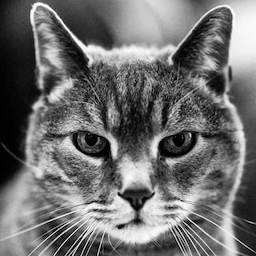
\includegraphics[width = 2in]{I.png}} &
\subfloat[$I^{(1)}$ - $f_1=\frac{1}{8}$]{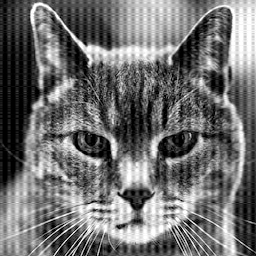
\includegraphics[width = 2in]{I1.png}}\\
\subfloat[$I^{(2)}$ - $f_2=\frac{1}{32}$]{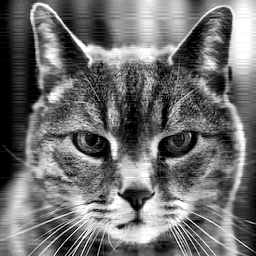
\includegraphics[width = 2in]{I2.png}} &
\subfloat[$I^{(12)}$ - $f_1,f_2$]{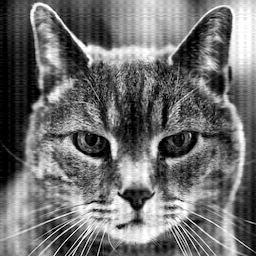
\includegraphics[width = 2in]{I12.png}}
\end{tabular}
\end{figure}

\subsection*{b}

Given a row of an image $I$. degraded by additive harmonic noise with fixed frequency but random iid amplitude and phase per row:
\begin{align*}
    I_{i,j}^{noisy} = I_{i,j} + A_i \cos (2\pi fj+\phi_i)
\end{align*}

\begin{align*}
    DFT(I^{noisy}_{row=k}) & = \sum_{j=0}^{columns=n} \frac{1}{\sqrt{n}} \exp \big( - \frac{2\pi ijk}{N} \big) \cdot I_{k,j}^{noisy} \\
    & = \sum_{j=0}^{n} \frac{1}{\sqrt{n}} \exp \big( - \frac{2\pi ijk}{N} \big) \cdot \big( I_{k,j} + A_k \cos (2\pi fj+\phi_k) \big) \\
    & = \underbrace{\sum_{j=0}^{n} \frac{1}{\sqrt{n}} \exp \big( - \frac{2\pi ijk}{N} \big) \cdot I_{k,j}}_{DFT(I_k)} + \underbrace{\sum_{j=0}^{n} \frac{1}{\sqrt{n}} \exp \big( - \frac{2\pi ijk}{N} \big) \cdot A_k \cos (2\pi fj+\phi_k)}_{DFT(noise)}
\end{align*}

The first term in the sum is simply the DFT of the original row, and the second term represents the DFT of the harmonic noise.

Since the amplitude and phase of the noise are random and independent for each row, the DFT of the noise will have random magnitude and phase. \\
This means that the DFT representation of the noisy columns (columns where the column number divides $1/f$) will have both the original signal and random harmonic noise present in the frequency domain.

\subsection*{c}

We consider having two harmonic noises now with frequencies $f_1 , f_2$, both dividing $n$, and the noise added to the image is the average of them.

\begin{align*}
    DFT(I_k^{noisy}) & = \sum_{j=0}^{n} \frac{1}{\sqrt{n}} \exp \big( - \frac{2\pi ijk}{N} \big) \cdot I_{k,j}^{noisy} \\
    & = \sum_{j=0}^{n} \frac{1}{\sqrt{n}} \exp \big( - \frac{2\pi ijk}{N} \big) \cdot \big( I_{k,j} + A_k \cos (2\pi f_1 j+\phi_k) + A_k^{\prime} \cos (2\pi f_2 j+\phi_k^{\prime}) \big) \\
    & = DFT(I_k) + DFT(\text{noise with }f_1) + DFT(\text{noise with }f_2)
\end{align*}

So, like the previous clause - since the amplitude and phase of the noise are random and independent for each row, the DFT of the noise
will have random magnitude and phase.

Also, the DFT representation of the noisy rows where the column number divides $\frac{1}{f_1}$ will have both the original signal and the first harmonic noise present.

In columns where the column number divides $\frac{1}{f_2}$ will have both the original signal and the second harmonic noise present. 

In columns where the column number divides both $\frac{1}{f_1}, \frac{1}{f_2}$ will have the original signal, the first and the second harmonic noise present in the frequency domain.

\newpage

\subsection*{d}

The empiric DFT is in the code. \\
The results of the imaginary and real parts of each image are:

\begin{figure}[h]
\begin{tabular}{cc}
\subfloat[$I$ real part]{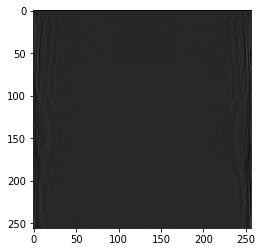
\includegraphics[width = 1.5in]{dft_0_real.png}} &
\subfloat[$I$ imaginary part]{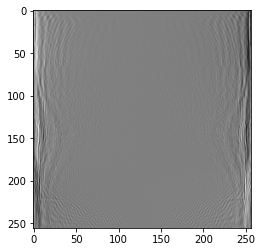
\includegraphics[width = 1.5in]{dft_0_imag.png}}\\
\subfloat[$I^{(1)}$ real part]{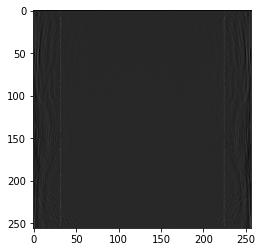
\includegraphics[width = 1.5in]{dft_1_real.png}} &
\subfloat[$I^{(1)}$ imaginary part]{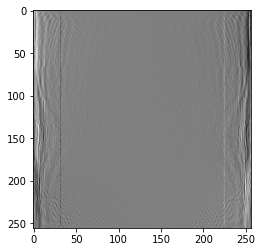
\includegraphics[width = 1.5in]{dft_1_imag.png}} \\
\subfloat[$I^{(2)}$ real part]{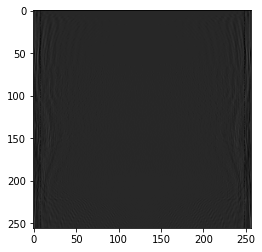
\includegraphics[width = 1.5in]{dft_2_real.png}} &
\subfloat[$I^{(2)}$ imaginary part]{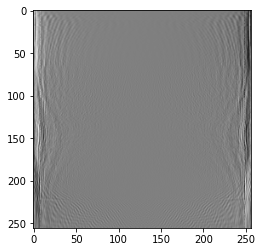
\includegraphics[width = 1.5in]{dft_2_imag.png}} \\ 
\subfloat[$I^{(12)}$ real part]{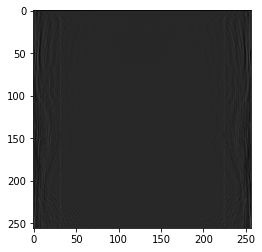
\includegraphics[width = 1.5in]{dft_12_real.png}} &
\subfloat[$I^{(12)}$ imaginary part]{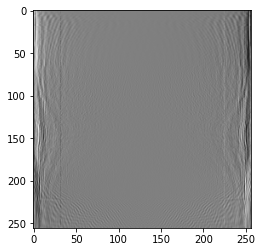
\includegraphics[width = 1.5in]{dft_12_imag.png}}
\end{tabular}
\end{figure}

\newpage
\subsection*{e}

We reconstructed the image from our noise-added images.\\
In $I^{(1)}$ we had $f_1=\frac{1}{8}$, and in $I^{(2)}$ we had $f_2=\frac{1}{32}$, so we zero out the in the noise frequency.

In $I^{(12)}$, our noise was the average of the two previous noises. To reconstruct that, we used two options -- each uses a reconstruction of $I^{(1)/(2)}$ and again reconstructs it with $f_{2/1}$.

The original image:

\begin{figure}[h]
    \centering
    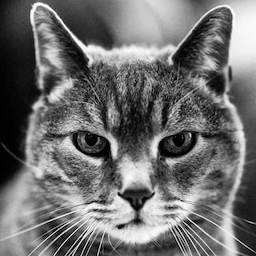
\includegraphics[width=2in]{I.png}
    \caption{$I$ -- Original image}
\end{figure}

The reconstructions:

\begin{figure}[h]
\centering
\begin{tabular}{cc}
\subfloat[$I^{(1)}$ reconstruction]{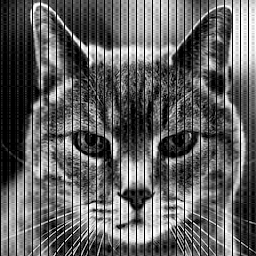
\includegraphics[width = 2in]{recon_1.png}} &
\subfloat[$I^{(2)}$ reconstruction]{
\includegraphics[width = 2in]{recon_2.png}}\\
\subfloat[$I^{(12)}$ reconstruction with $I^{(2)}$ first]{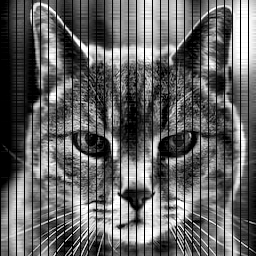
\includegraphics[width = 2in]{recon_12_1.png}} &
\subfloat[$I^{(12)}$ reconstruction with $I^{(1)}$ first]{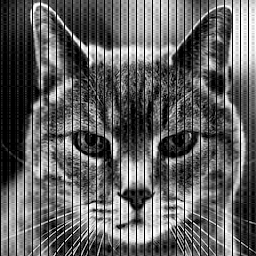
\includegraphics[width = 2in]{recon_12_2.png}}
\end{tabular}
\end{figure}

\newpage
And the MSE:

\begin{table}[h]
    \centering
    \begin{tabular}{c|c}
        $I^{(1)}$ MSE & 87.473 \\
        $I^{(2)}$ MSE & 84.277 \\
        $I^{(12)}$ MSE & 74.593 \\
        $I^{(1)}$ recon MSE & 88.589 \\
        $I^{(2)}$ recon MSE & 84.274 \\
        $I^{(12)}$ recon with $I^{(1)}$ first MSE & 88.589 \\
        $I^{(12)}$ recon with $I^{(2)}$ first MSE & 85.348
    \end{tabular}
\end{table}

As we can see - we got higher MSE with $I^{(1)}$ as expected since we zero out more pixels.
Zeroing-out columns in $I^{(1)}$ did not help, as zeroing out every 32 column does nothing if each 8th column is zero.

This de-noising process did little, as we can see that for $I^{(1)}$ and $I^{(12)}$ the process only made the MSE higher, and only did a miniscule change in $I^{(2)}$.

All-in-all, we zeroed-out the noise frequencies but got little in return in terms of MSE.

\end{document}